% Author: Till Tantau
% Source: The PGF/TikZ manual
\documentclass{article}

\usepackage[latin1]{inputenc}
\usepackage{tikz}

% GNUPLOT required
\begin{document}
\pagestyle{empty}


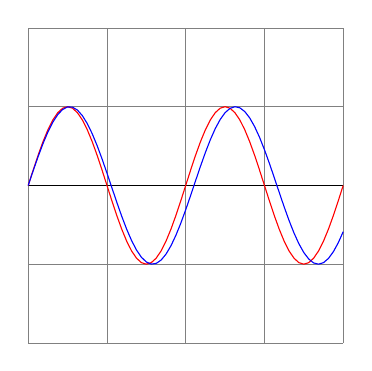
\begin{tikzpicture}[domain=0:4]
    \draw[very thin,color=gray] (0,-2) grid (4,2);
    \draw[-] (0,0) -- (4,0); 
    \draw[red, samples=65] plot (\x, {sin(pi*\x*1 r)});
    \draw[blue, samples=65] plot(\x, {sin(pi*\x*.950 r)});
    \end{tikzpicture}


\end{document}
